\subchapter{Describing Hardware Devices}
{Objective: learn how to describe hardware devices.}

\section{Goals}

Now that we covered the Device Tree theory, we can explore the list of
existing devices and make new ones available. In particular, we will
create a custom Device Tree to describe the few extensions we will make
to our BeaglePlay board.

\section{Setup}

Go to the \code{~/__SESSION_NAME__-labs/src/linux} directory. Check out the
\code{6.7.bootlin} branch.

Now create a new \code{beagleplay-custom} branch starting from this branch,
for your upcoming Device Tree changes on the Beagle Play.

Download a useful document sharing useful details about the Nunchuk
and its connector:\\
\url{https://bootlin.com/labs/doc/nunchuk.pdf}

\section{Create a custom device tree}

To let the Linux kernel handle a new device, we need to add a
description of this device in the board device tree.

As the Beagle Play device tree is provided by the kernel community,
and will continue to evolve on its own, we don't want to make changes
directly to the device tree file for this board.

The easiest way to customize the board DTS is to create a new DTS file
that includes the Beagle Play DTS, and adds its own definitions.

So, create a new
\code{arch/arm64/boot/dts/ti/k3-am625-beagleplay-custom.dts} file in which
you just include the regular board DTS file. We will add further
definitions in the next sections.

\begin{verbatim}
// SPDX-License-Identifier: GPL-2.0
#include "k3-am625-beagleplay.dts"
\end{verbatim}

Modify the \kfile{arch/arm64/boot/dts/ti/Makefile} file to add your custom
Device Tree, and then have it compiled with (\code{make dtbs}). Now,
copy the new DTB to the tftp server home directory, change the DTB file
name in the U-Boot configuration\footnote{Tip: you just need to run
\code{editenv bootcmd} and \code{saveenv}.}, and boot the board.

\section{Setting the board's model name}

Modify the custom Device Tree file to override the model name for your
system. Set the \code{model} property to \code{Training Beagle Play}. Don't hesitate to ask your instructor if you're not sure how.

Recompile the device tree, and reboot the board with it. You should see
the new model name in two different places:

\begin{itemize}
\item In the first kernel messages on the serial console.
\item In \code{/sys/firmware/devicetree/base/model}. This can be
      handy for a distribution to identify the device it's running on.
\end{itemize}

\section{Driving LEDs}

The BeaglePlay features five user LEDs (\code{LED_USR0}, \ldots, \code{LED_USR4})
in the corner near the USB-C port.

Start by looking at the different description files and look for a node
that would be defining the LEDs.

The five LEDs are actually supposed to be triggered by a driver matching
the compatible \code{gpio-leds}. This is a generic driver which acts on
LEDs connected to GPIOs. But as you can observe, despite being part of
the in-use Device Tree, the LEDs remain off. The reason for that is the
absence of driver for this node: nothing actually drives the LEDs even
if they are described. So you can start by recompiling your kernel with
\kconfigval{CONFIG_LEDS_GPIO}{y}.

You should now see \code{USR_LED0} blink with the CPU activity, \code{USR_LED1}
staying on, and the others staying off. If you look at the bindings documents
\kfile{Documentation/devicetree/bindings/leds/common.yaml} and
\kfile{Documentation/devicetree/bindings/leds/leds-gpio.yaml}, you'll notice we
can tweak the \code{default-state} in order to make the three inactive user
LEDs bright.

You will need to modify a shared DTSI file in order to do that. But
because we do not want to impact other boards also using that same DTSI
file, we might instead add a label to the \code{leds} container node. We
could then reference this new label in our custom DTS and overwrite the
\code{default-state} property of each LED subnode.

Reboot the board using the new DTS and observe the LEDs default states change.
If you look again at the common file defining the LEDs, they are actually all
linked to a \code{linux,default-trigger}. The default state only applies until
the trigger starts its activity.

\code{USR_LED0} is a heartbeat which you can enable or disable with
\kconfig{CONFIG_LEDS_TRIGGER_HEARTBEAT}. \code{USR_LED1} is triggered by disk
activity.

\section{Managing I2C buses and devices}

The next thing we want to do is connect an Nunchuk joystick
to an I2C bus on our board. The I2C bus is very frequently used
to connect all sorts of external devices. That's why we're covering
it here.

\subsection{Enabling an I2C bus}

As shown on the below picture found on
\url{https://docs.beagleboard.org/latest/boards/beagleplay/03-design.html}, the
BeaglePlay has 3 I2C busses available through different connectors:

\begin{itemize}
\item I2C3: available on the mikroBUS connector
\item I2C1: available on the Grove connector
\item I2C2: available on the Qwiic connector
\end{itemize}

The AM62x SoC has three others I2C controllers, but they are not used on the
BeaglePlay board. However because the default device-tree we are using enables
all the I2C controllers except one, we expect the kernel to detect five I2C
buses in total.

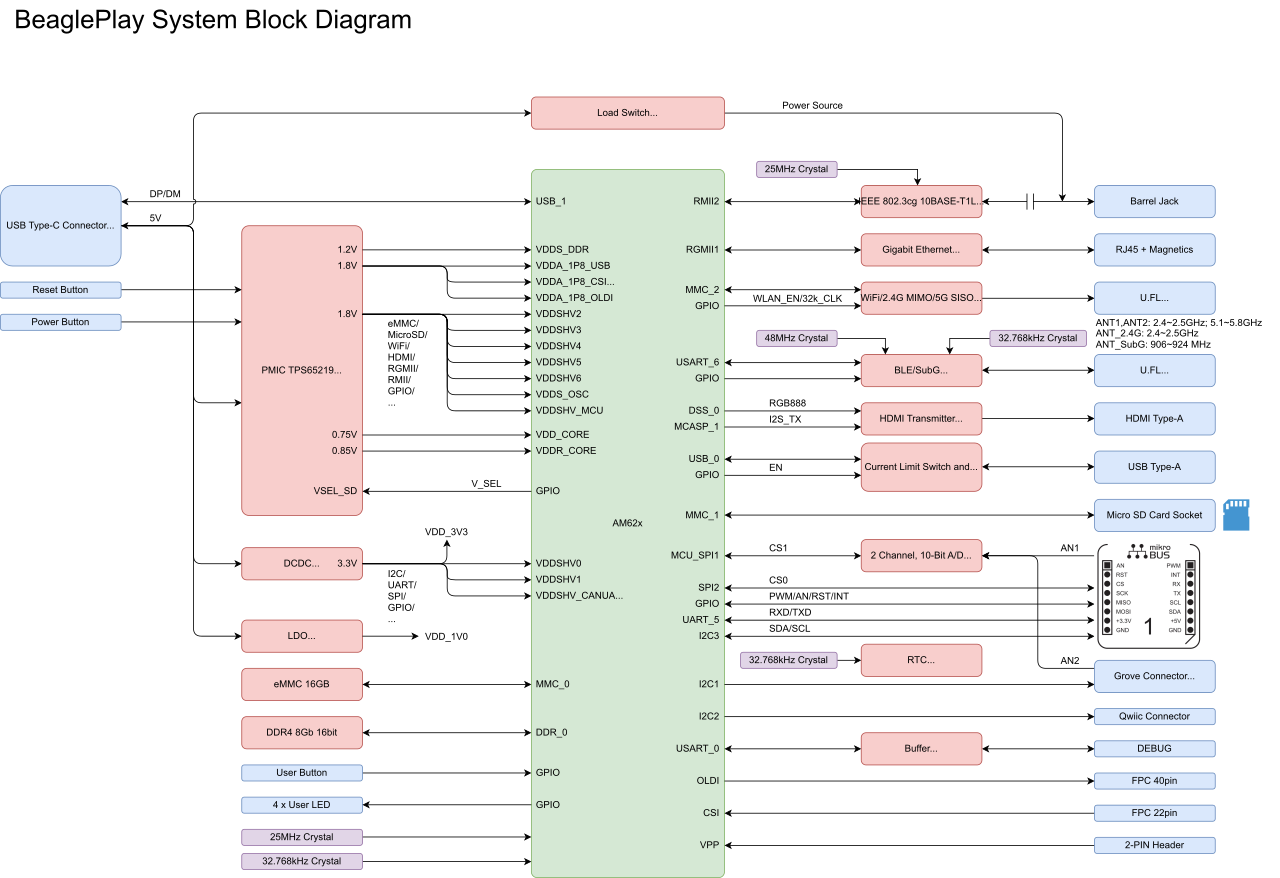
\includegraphics[width=\textwidth]{labs/sysdev-accessing-hardware-beagleplay/System-Block-Diagram.png}

In this lab we will be using the I2C3 bus to connect the nunchuk because it is
located on the mikroBUS connector and is easily accessible.

So, let's see which I2C buses are already enabled:

\begin{bashinput}
# i2cdetect -l
i2c-3 i2c OMAP I2C adapter I2C adapter
i2c-1 i2c OMAP I2C adapter I2C adapter
i2c-2 i2c OMAP I2C adapter I2C adapter
i2c-0 i2c OMAP I2C adapter I2C adapter
i2c-5 i2c OMAP I2C adapter I2C adapter
\end{bashinput}

As the bus numbering scheme in Linux doesn't always match the one
on the datasheets, let's check the base addresses of the registers
of these controllers:

\begin{bashinput}
# ls -l /sys/bus/i2c/devices/i2c-*
lrwxrwxrwx 1 root root 0 Jan 1 02:02 /sys/bus/i2c/devices/i2c-0 -> ../../../devices/platform/\
bus@f0000/20000000.i2c/i2c-0
lrwxrwxrwx 1 root root 0 Jan 1 02:02 /sys/bus/i2c/devices/i2c-1 -> ../../../devices/platform/\
bus@f0000/20010000.i2c/i2c-1
lrwxrwxrwx 1 root root 0 Jan 1 02:02 /sys/bus/i2c/devices/i2c-2 -> ../../../devices/platform/\
bus@f0000/20020000.i2c/i2c-2
lrwxrwxrwx 1 root root 0 Jan 1 02:02 /sys/bus/i2c/devices/i2c-3 -> ../../../devices/platform/\
bus@f0000/20030000.i2c/i2c-3
lrwxrwxrwx 1 root root 0 Jan 1 02:02 /sys/bus/i2c/devices/i2c-5 -> ../../../devices/platform/\
bus@f0000/bus@f0000:bus@4000000/4900000.i2c/i2c-5
\end{bashinput}

Interpreting this output is not completely straightforward, but you can suppose
that:

\begin{itemize}
\item I2C0 is at address \code{0x20000000}
\item I2C1 is at address \code{0x20010000}
\item I2C2 is at address \code{0x20020000}
\item I2C3 is at address \code{0x20030000}
\item I2C5 is at address \code{0x04900000}
\end{itemize}

Now let's double check the addressings by looking at the
\href{https://www.ti.com/lit/ug/spruiv7a/spruiv7a.pdf}{TI AM62x SoC
datasheet}, in the \code{Memory Map} section:

\begin{itemize}
\item I2C0 is indeed at address \code{0x20000000}
\item I2C1 is indeed at address \code{0x20010000}
\item I2C2 is indeed at address \code{0x20020000}
\item I2C3 is indeed at address \code{0x20030000}
\item I2C4 doesn't exist in the reference manual but corresponds to
      WKUP\_I2C0 at address \code{0x2b200000}
\item I2C5 doesn't exist in the reference manual but corresponds to
      MCU\_I2C0 at address \code{0x04900000}
\end{itemize}

So luckily, the first 4 Linux I2C names correspond to the first 4 datasheet
names.

\subsection{Prepare the I2C device DT description}

Before describing your nunchuk device, let's think about what will be
needed:
\begin{itemize}
\item The device node should follow a standard pattern.

  The node name should be \code{joystick@addr}, the convention for node
  names is \code{<device-type>@<addr>}.

\item We want to be able to fully identify the programming model.

  This is usually done using a unique compatible string. The compatible
  contains a vendor prefix and then a more specific string. We will use
  \code{nintendo,nunchuk}.

\item We need to identify how to reach the device.

  This is the \code{reg} property and we should set it to the I2C
  address of the nunchuk. You will find the I2C slave address of the
  Nunchuk on the nunckuk document that we have downloaded
  earlier\footnote{This I2C slave address is enforced by the device
    itself. You can't change it.}.

\item (Optional) There are two types of nunchuks.

  There are white and black nunchuks, which don't expect the same
  initialization flow. We could imagine a boolean property named
  \code{nintendo,alternate-init} which will change the initialization
  logic. See the nunchuk pdf for details about the alternate flow.

\end{itemize}

Stopping here is sufficient as writing device-tree bindings is not
strictly required to continue the labs, but if you feel comfortable
you may want to write your own binding file, eg:
\begin{bashinput}
Documentation/devicetree/bindings/misc/nintendo,nunchuk.yaml
\end{bashinput}
Once you are confident with your bindings, you can even copy the
examples from the \code{wrong-nunchuk-examples.yaml} (in the
\code{nunchuk} labs folder) inside your bindings and verify they all
pass/fail as expected!
\begin{bashinput}
make DT_SCHEMA_FILES=misc/nintendo,nunchuk.yaml dt_binding_check
\end{bashinput}

\subsection{Declare the Nunchuk device}

As a child node to the \code{i2c3} bus, now declare an I2C device
for the Nunchuk, following the above rules.

If you wrote an optional YAML binding, you can also double check your
node:
\begin{bashinput}
make DT_SCHEMA_FILES=misc/nintendo,nunchuk.yaml dtbs_check
\end{bashinput}

After updating the running Device Tree, explore
\code{/sys/firmware/devicetree}, where every subdirectory corresponds to
a DT node, and every file corresponds to a DT property. You can search
for presence of the new \code{joystick} node:

{\small
\begin{verbatim}
# find /sys/firmware/devicetree -name "*joystick*"
/sys/firmware/devicetree/base/bus@f0000/i2c@20030000/joystick@52
\end{verbatim}
}

You can also check the whole structure of the loaded Device Tree, using
the Device Tree Compiler (\code{dtc}), which we put in the root
filesystem:
\begin{verbatim}
# dtc -I fs /sys/firmware/devicetree/base/ > /tmp/dts
# grep -C10 nunchuk /tmp/dts
\end{verbatim}

Once your new Device Tree seems correct, commit your changes. As you
modified a shared file and a custom file, it is good practice to commit
these changes in two different patches.
